\section{Servlet}

\texttt{javax.servlet.Servlet} ist das Interface, das letztendlich entscheidet, ob eine Java-Klasse überhaupt ein Servlet ist. Jedes Servlet muss dieses Interface direkt oder indirekt implementieren. De facto wird man aber wohl in den meisten Fällen nicht das Interface selber implementieren, sondern auf \texttt{javax.servlet.GenericServlet} (falls man kein Servlet für HTTP-Anfragen schreibt), bzw. \texttt{javax.servlet.http.HttpServlet} für http-Anfragen zurückgreifen. HttpServlet implementiert alle wesentlichen Methoden bis auf die http-doXXX-Methoden wie doGet oder doPost. Man muss nur noch die Methoden doGet, doPost oder `doXYZ überschreiben, je nachdem, welche HTTP-Methoden man unterstützen will.

\begin{minted}[breaklines]{java}
public class BasicServlet extends HttpServlet {

    enum Directories {questionnaires, funny}

    protected void doGet(HttpServletRequest request, HttpServletResponse response) throws IOException {

        response.setContentType("text/html; charset=utf-8");

        String[] pathElements = request.getPathInfo().split("/");
        Arrays.stream(pathElements).forEach(log::debug);

        if (pathElements.length > 0) {

            if (Arrays.stream(Directories.values()).anyMatch(d -> d.name().equals(pathElements[1]))) {

                switch (Directories.valueOf(pathElements[1])) {
                    case questionnaires:
                        Long id = pathElements.length == 3 ? Long.valueOf(pathElements[2]) : null;
                        // Path contains ID
                        if (id != null) {
                            handleSingleQuestionaire(id, request, response);
                        } else {
                            handleQuestionaires(request, response);
                        }
                        return;
                    default:
                        handleRoot(request, response);

                }
            } else {
                handelDefault(request, response);
            }
        } else {
            handleRoot(request, response);
        }
    }

    private void handleSingleQuestionaire(Long id, HttpServletRequest request, HttpServletResponse response) throws IOException {
       ...
    }

    private void handleQuestionaires(HttpServletRequest request, HttpServletResponse response) throws IOException {
        QuestionnaireRepository questionnaireRepository = (QuestionnaireRepository) request.getServletContext().getAttribute(QuestionnaireRepository.class.getName());
        PrintWriter writer = response.getWriter();
        writer.append(HTML_HEAD);
        writer.append("<h3>{questionnaires}</h3>");
        List<Questionnaire> questionnaires = questionnaireRepository.findAll();
        questionnaires.forEach(questionnaire -> {
            final String url = request.getContextPath() + request.getServletPath() + "/questionnaires/" + questionnaire.getId().toString();
            writer.append(String.format("<p><a href='%s'>%s</a></p>", response.encodeURL(url), questionnaire.getTitle()));
        });
        writer.append(HTML_BODY_END);
    }

    private void handleRoot(HttpServletRequest request, HttpServletResponse response) throws IOException {
       ...
    }
}
\end{minted}
\subsection{Servlet Container}
Der Servlet Container stellt eine Umgebung zur Verfügung indem die Servlets laufen gelassen werden können. Der Container sorgt zunächst einmal für den korrekten Lebenszyklus der Servlets. Zumeist arbeitet der Container im Zusammenspiel mit einem Webserver.

\subsubsection{Laden der Servlet Klasse}
Zunächst muss der Classloader des Containers die Servlet-Klasse laden. Wann der Container dies macht, bleibt ihm überlassen, es sei denn, man definiert den entsprechenden Servlet-Eintrag im Deployment-Deskriptor. Mit dem optionalen Eintrag «load-on-startup» wird definiert, dass der Servlet-Container die Klasse bereits beim Start des Containers lädt. Die Zahlen geben dabei die Reihenfolge vor (Servlets mit niedrigeren «load-on-startup»-Werten, werden früher geladen).

\subsection{Servlet Request und Response}
In den Verarbeitungsmethoden von Servlets (\texttt{service()}, \texttt{doGet()}, \texttt{doPost()}…) hat man stets Zugriff auf ein Objekt vom Typ ServletRequest. Arbeitet man mit HttpServlet handelt es sich um das Interface  \texttt{javax.servlet.http.HttpServletRequest}, ansonsten um das Interface \texttt{javax.servlet.ServletRequest}. Diese Interfaces stellen wesentliche Informationen über den Client-Request zur Verfügung.
\subsection{ServletContext}
Jedes Servlet wird im Kontext der Webapplikation ausgeführt. Dieser Kontext gilt für alle Servlets der entsprechenden Webapplikation. Deshalb werden Informationen, die im Scope der Webapplikation gelten hier abgelegt, so dass jedes Servlet auf diese zugreifen kann.

\begin{minted}{bash}
    |-- src
    |-- main
    |   |-- java
    |   |   |-- ch
    |   |       |-- fhnw
    |   |           |-- webfr
    |   |               |-- flashcard
    |   |                   |-- domain
    |   |                   |   |-- Questionnaire.java
    |   |                   |-- filter
    |   |                   |   |-- BasicFilter.java
    |   |                   |   |-- TranslationFilter.java
    |   |                   |-- listener
    |   |                   |   |-- BasicListener.java
    |   |                   |-- persistence
    |   |                   |   |-- QuestionnaireRepository.java
    |   |                   |-- util
    |   |                   |   |-- QuestionnaireInitializer.java
    |   |                   |-- web
    |   |                       |-- BasicServlet.java
    |   |-- resources
    |   |   |-- log4j.properties
    |   |   |-- messages.properties
    |   |-- webapp
    |       |-- WEB-INF
    |       |   |-- web.xml
    |       |-- css
    |       |   |-- styles.css
    |       |-- smiley.png
    |-- test
\end{minted}
\subsection{web.xml}
Konfigurationsfile für die Webapp. Das File wird beim Hochfahren der Webapp vom Web-Container gelesen, um die Webapp entsprechend zu konfigurieren.
\begin{minted}[breaklines]{xml}
<?xml version="1.0" encoding="ISO-8859-1" standalone="no"?>
<web-app xmlns="http://java.sun.com/xml/ns/javaee" xmlns:xsi="http://www.w3.org/2001/XMLSchema-instance" version="3.0"
         xsi:schemaLocation="http://java.sun.com/xml/ns/javaee http://java.sun.com/xml/ns/javaee/web-app_3_0.xsd">
 
    <display-name>Basic Servlet Web Application</display-name>
    <servlet>
        <servlet-name>Basic Servlet</servlet-name>
        <servlet-class>ch.fhnw.webfr.flashcard.web.BasicServlet</servlet-class>
    </servlet>
    <servlet-mapping>
        <servlet-name>Basic Servlet</servlet-name>
        <url-pattern>/*</url-pattern>
    </servlet-mapping>
    <filter>
        <filter-name>Basic Filter</filter-name>
        <filter-class>ch.fhnw.webfr.flashcard.filter.BasicFilter</filter-class>
    </filter>
    <filter-mapping>
        <filter-name>Basic Filter</filter-name>
        <url-pattern>/*</url-pattern>
    </filter-mapping>
    <listener>
        <listener-class>ch.fhnw.webfr.flashcard.listener.BasicListener</listener-class>
    </listener>
    <context-param>
        <param-name>mode</param-name>
        <param-value>test</param-value>
    </context-param>
</web-app>
\end{minted}
\subsection{Filter}
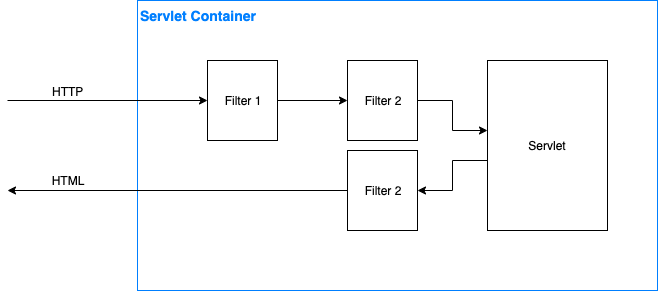
\includegraphics[width=\columnwidth]{images/filter}
Servlet-Filter bieten eine Möglichkeit auf Request und Response zwischen Client und Servlet zuzugreifen. Dabei können mehrere Filter eine Filterkette bilden. Dabei wird mittels Mapping-Regeln bestimmt, welche Filter für welche Requests wann zuständig sind. Es gibt zahlreiche Möglichkeiten, bei denen der Einsatz eines Filters sinnvoll sein kann. Der einfachste Anwendungsfall ist das Tracing, um zu sehen welche Ressource angesprochen wurde und wie lange die Bereitstellung der Ressource gedauert hat. Weitere typische Anwendungsfälle umfassen die Security bspw. eine Entschlüsselung des Requests und die Verschlüsselung der Response. Filter sind im Deployment-Descriptor deklariert (oder über die Annotation \texttt{@WebFilter}). Sie werden vom Container verwaltet und müssen das Interface \texttt{javax.servlet.Filter} implementieren. Es gibt drei Methoden, die den Lifecycle bestimmen: 
\begin{itemize}
\item \texttt{init(FilterConfig)} - wird aufgerufen, nachdem der Container die Instanz der Filterklasse erzeugt hat
\item \texttt{doFilter(ServletRequest, ServletResponse, FilterChain)} - wird bei der Abarbeitung der FilterChain gerufen 
\item \texttt{destroy()} - die Filterinstanz wird gleich beseitig
\end{itemize}
\subsubsection{Interceptor Pattern}
Interceptors sollen technische Dienste bereitstellen, die nicht direkt mit der Anwendungslogik zu tun haben.

\subsubsection{Chain of Responsibility}
Pattern Der Auslöser und der Verarbeiter einer Nachricht werden entkoppelt. Es wird dabei eine Kette von Objekten durchlaufen, welche die Nachricht verarbeiten können. Die Nachricht wird solange weitergereicht, bis ein Objekt diese verarbeitet hat oder das Ende der Kette erreicht ist.
\subsubsection{Filter Mapping}
Die Reihenfolge der Filter wird im \texttt{web.xml} definiert.
Die Reihenfolge kann nicht über Annotationen gemacht werden.
\begin{minted}[breaklines]{java}
public class BasicListener implements ServletContextListener {
 
    enum Mode {test,prod}
 
    @Override
    public void contextInitialized(ServletContextEvent sce) {
        ServletContext ctx = sce.getServletContext();
        Object attribute = ctx.getInitParameter("mode");
        try {
            Mode mode = Mode.valueOf(String.valueOf(attribute));
            log.info("Mode: {}", mode.name());
            switch (mode) {
                case test:
                    QuestionnaireRepository questionnaireRepository = new QuestionnaireInitializer().initRepoWithTestData();
                    ctx.setAttribute(QuestionnaireRepository.class.getName(), questionnaireRepository);
                    log.info("Test Repository initialized and set.");
                    break;
                case prod:
                    // init prod repo 
                    break;
                default:
                    log.info("No mode set.");
            }
        } catch (IllegalArgumentException e) {
            log.error("Invalid mode {}", attribute);
        }
    }
}
\end{minted}
\subsection{Response Modification}
Es ist auf dem Outbound nicht möglich den Original Response direkt zu manipulieren, da mit dem Abschluss der service()-Methode im Servlet der Servlet-Container implizit ein flush() und close() auf den OutputStream aufruft. Somit ist eine Modifikation ausgeschlossen - und deshalb kommen die folgenden Wrapper Klassen in Spiel:
\begin{itemize}
\item HttpServletResponseWrapper: Provides a convenient implementation of the HttpServletResponse interface that can be subclassed by developers wishing to adapt the response from a Servlet.
\item HttpServletRequestWrapper: Provides a convenient implementation of the HttpServletRequest interface that can be subclassed by developers wishing to adapt the request to a Servlet.
\end{itemize}
\begin{minted}[breaklines]{java}
@Slf4j
public class TranslationFilter implements Filter {

    public void doFilter(ServletRequest request, ServletResponse response, FilterChain chain) throws IOException, ServletException {

        log.debug("TranslationFilter doFilter!");

        ServletResponse newResponse = response;

        if (request instanceof HttpServletRequest) {
            newResponse = new CharResponseWrapper((HttpServletResponse) response);
        }

        chain.doFilter(request, newResponse);

        if (newResponse instanceof CharResponseWrapper) {
            String text = newResponse.toString();
            log.debug(text);
            if (text != null) {
                Locale currentLocale = Locale.forLanguageTag(request.getServletContext().getInitParameter("lang"));
                log.info("Language: {}", currentLocale);
                ResourceBundle resourceBundle = ResourceBundle.getBundle("messages", currentLocale);

                Map<String, String> texts = resourceBundle.keySet().stream().collect(Collectors.toMap(k -> k, resourceBundle::getString));
                String translatedText = StrSubstitutor.replace(text, texts, "{", "}");
                log.debug(translatedText);
                response.getWriter().write(translatedText);
                response.setContentLength(translatedText.length());
            }
        }

    }

\end{minted}
\begin{minted}[breaklines]{java}
    @Override
    public void init(FilterConfig fConfig) {
        log.debug("TranslationFilter init!");
    }

    @Override
    public void destroy() {
        log.debug("TranslationFilter destroy!");
    }

    class CharResponseWrapper extends HttpServletResponseWrapper {
        protected CharArrayWriter charWriter;

        protected PrintWriter writer;

        protected boolean getOutputStreamCalled;

        protected boolean getWriterCalled;

        public CharResponseWrapper(HttpServletResponse response) {
            super(response);

            charWriter = new CharArrayWriter();
        }

        public ServletOutputStream getOutputStream() throws IOException {
            if (getWriterCalled) {
                throw new IllegalStateException("getWriter already called");
            }

            getOutputStreamCalled = true;
            return super.getOutputStream();
        }

        public PrintWriter getWriter() throws IOException {
            if (writer != null) {
                return writer;
            }
            if (getOutputStreamCalled) {
                throw new IllegalStateException("getOutputStream already called");
            }
            getWriterCalled = true;
            writer = new PrintWriter(charWriter);
            return writer;
        }

        public String toString() {
            String s = null;

            if (writer != null) {
                s = charWriter.toString();
            }
            return s;
        }
    }

}
\end{minted}